% !TEX root = NotesDeCours.tex



\begin{frame}

  \color{bleu}

  \begin{flushleft}
    
    \Large
   	\bf
    
    Mécanique des fluides 	
    
  \end{flushleft}
  
  \ligne{3} % remplace: \noindent \thickline{0.5mm}{150}

  \begin{flushright}

    \rm

    \textrm{David} \textsc{Fabre}
    
    \vspace{3mm}
    
    IMFT / UPS
    
    Département de Mécanique
    
david.fabre@imft.fr

  \end{flushright}


  \begin{picture}(110, 30)(10, -20)
%    \put(15, -17){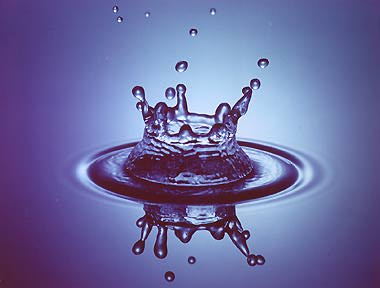
\includegraphics[height=42mm]{./Figures/splash.jpg}}
 \put(15, -17){\includegraphics[height=42mm]{../FIGURES/Wasa.jpg}}
  \end{picture}

  \vspace{2mm}
  
  \begin{flushright}
    
    \Large
   	\bf
    
    2. Forces de pression dans un fluide -- Hydrostatique

  \end{flushright}


\end{frame}



\handout{
\begin{frame}{Sommaire}
\small  
\hspace*{2mm}
\begin{tabular}{cc}
		%&
  		\begin{minipage}{62mm}
  			\tableofcontents[]
      \vspace{15mm}
  		\end{minipage}
  		&   
  		\begin{minipage}{60cm}
		  \vspace*{-5mm}  
  			%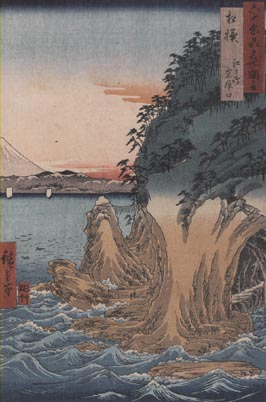
\includegraphics[width=40mm]{vagues.jpg} 
  		\end{minipage}
  	\end{tabular}
\vspace{0mm}
\end{frame}
}

%\setcounter{section}{1}
\nohandout{\section{Forces de pression dans un fluide -- Hydrostatique}}

\subsection{ Pression (et température) : signification physique. 
} 


%\subsubsection{Description d'un fluide (II) : point de vue microscopique}


%--------------------------------------------------------------------------------------------------


%%%%%%%%%%%%%%%%%%%%%
\begin{frame}{Pression : définition(s)}

\small

Définitions : 

\begin{itemize}[<+-| alert@+>]
\item Définition Thermodynamique : (pour un système simple)

Pression = variable intensive reliée aux échanges d'énergie mécaniques 
(liée au mouvement d'une frontière, et donc à la modification du volume) 

$$
p = - {\left( \frac{\partial E}{\partial V} \right)}_{S} = \rho {\left( \frac{\partial e}{\partial \rho} \right)}_{s} 
$$  


(Définition théorique mais inutilisable avec les modèles de fluides les plus courants, pour lesquels $e = e(T,P)...$)

Corollaire : à l'équilibre thermodynamique $p$ est uniforme ; cf. cours thermo.


\item Définition mécanique 

Pression = force surfacique normale exercée par un fluide au repos sur une surface matérielle (frontière avec une paroi solide)
 ou fictive (séparant avec un autre domaine fluide).

En considérant une {\em surface élémentaire} (au sens de la MMC) $dS$ de normale $\vec{n}_{{\cal F} \rightarrow {\cal S} }$, la force élémentaire exercée par le fluide sur la surface vaut 

$$
d \vec{f}_{{\cal F} \rightarrow {\cal S} } = p  \vec{n}_{{\cal F} \rightarrow {\cal S} } d S
$$

\pause

\color{gris}{
\tiny
 Lien entre les 2 définitions :

En supposant que la surface $\cal S$ subit un déplacement {\em élémentaire}  (au sens de la thermo) $\delta \vec X$, le travail reçu par le fluide vaut:

$$
\delta W = \iint_{\cal S} \delta \vec{X} \cdot (p  \vec{n}_{{\cal S} \rightarrow {\cal F} } d S )
$$

En supposant la pression uniforme il vient $\delta W = - p dV$ avec $dV = 
\iint_{\cal S} \delta \vec{X} \cdot \vec{n}_{{\cal F} \rightarrow {\cal S} } d S$.

} 

\pause 
\item Définition cinétique :

La pression est un {\em flux surfacique de quantité de mouvement microscopique normale} transféré par les particules à une paroi ou à un domaine fluide adjacent.



\end{itemize}


\end{frame}


\begin{frame}{Notions de théorie cinétique}
%--------------------------------------------------------------------------------------------------

\small

%Point de vue microscopique (échelle microscopique $\ell$) : 

%Description individuelle du mouvement des particules (masse $m_i$, vitesse $\vec{v}_i(t)$).



Sous l'hypothèse du milieu continu $Kn \ll 1$ (cf. chap. 1), 
on peut faire des moyennes sur le VER et définir successivement :

\smallskip 
\pause
- La masse volumique

$$
\rho = \frac{ N m_p}{V}   ,
$$

\pause 
- La vitesse moyenne 
$$
\vec{u} = \frac{1}{N} \sum_{i \in V} \vec{v}_i  ,
$$



\pause
- La vitesse quadratique moyenne 


$$
v_q^2 =  \frac{1}{N} \sum_{i \in V} \frac{| \vec{v_i} - \vec{u}|^2}{2}
$$

\pause 
Cette dernière quantité permet de définir la Température cinétique :

$$
T = \frac{ m_p v_q^2}{3 k_b}  \qquad ( k_B = 1.38 \cdot  10^{-23} m^2 kg s^{-2} K^{-1} \mbox{constante de Boltzmann} )
$$  
 

Remarque : 
on peut aussi écrire cette relation sous une forme plus pratique à l'échelle macroscopique :

$$
T = \frac{ M v_q^2}{3 R}  =  \frac{v_q^2}{3 r}
$$


%\pause

%\medskip

%On peut par ailleurs définir une échelle microscopique $\ell$ %caractérisant les interactions entre particules.


\end{frame}




%%%%%%%%%%%%%%%%%%%%%%%%%%%%%%%
\begin{frame} {Origine physique de la pression : cas des gaz}

\small 

Dans un gaz {\em parfait} les particules n'interagissent que par des collisions (sur une paroi ou entre elles).


%a pression est une variation de {\em quantité de mouvement normale} 
%liée aux collisions (sur une surface solide) ou aux particules traversant la surface (pour une surface entre deux domaines fluides adjacents).
\medskip

{\color{vert} Illustrations avec le programme kinetics.m}

\pause
\medskip 

%Pression = (densité) x (agitation thermique).

%c.a.d. $p = \rho r T$ (loi des gaz parfaits)

La théorie cinétique permet de calculer $p$ en fonction des propriétés microscopiques (cf. Guyon, Hulin, Petit ; cours Thermo L2).

\medskip

Calcul simplifié de la force de pression exercé sur une paroi 
(identifée à la variation de qdm due aux impacts sur celle-ci) :


$$
p =   \underbrace{\frac{n}{6} v_q}_{\mbox{ flux de particules impactant la paroi}}  \times  \underbrace{ 2 m_p v_q}_{\mbox{ variation de qdm au cours d'un impact}}
$$

où $n=N/V = \rho/m_p$ est la densité volumique de particules.

Ce qui aboutit à l'équation d'état mécanique :

$$
p = \rho r T
$$

\smallskip





\pause
\bigskip

{\bf Remarque :} 

Dans un gaz, l'échelle microscopique $\ell$ caractérisant les interactions interparticules est le  "libre parcours moyen" 

$$\ell  = \frac{1}{n \pi a^2}  $$ 

où $n = \frac{N}{V} = \frac{\rho}{m_p}$ est la densité volumique de particules et $a$ le rayon "effectif" des particules (rayon efficace de choc).

Ordres de grandeur : $a \approx 0.1 nm = 10^{-10} m$; 
 $\ell \approx 100 nm $ (dans l'air à température et pression ambiantes).
 






\end{frame}

%%%%%%%%%%%%%%%%%%%%%%%%%%%%%%%%%%%%
\begin{frame} {Origine physique de la pression : cas des liquides}

\small 
Dans un liquide la pression est due aux liaisons (répulsives ou attractives) entre les molécules adjacentes.

\smallskip

La pression dans un liquide peut ainsi être négative (liaisons majoritairement attractives).

Cet état est métastable du point de vue thermo mais qui peut tout de même être observé dans la nature (sève dans les arbres de plus de 10m...)

\medskip

NB : les liaisons sont très "raides" et il est difficile de faire varier la distance inter-molécule.

Ceci justifie que les liquides sont très peu compressibles. 

\smallskip

Modèle "liquide incompressible, indilatable" : $\rho = \rho_0 = C_{te}$ . 

$\partial \rho / \partial p \approx 0 $ $\rightarrow$ $\rho$ et $p$ sont découplés.  

Dans ce modèle $p$ devient une variable mécanique qui n'est plus reliée à la thermodynamique.



\pause
\bigskip

{\bf Remarque :} 

Dans un liquide, l'échelle microscopique $\ell$ caractérisant les interactions interparticules est la distance inter-moléculaire

$$\ell  = n^{-1/3}  $$ 

où $n = \frac{N}{V} = \frac{\rho}{m_p}$ est la densité volumique de particules.

Ordre de grandeur :  $\ell \approx 1 nm $ 
 






\end{frame}

\subsection{Hydrostatique}

\subsubsection{Loi de l'hydrostatique}

%%%%%%%%%%%%%%%%%%%%%%%%%%%%%%
%--------------------------------------------------------------------------------------------------
\begin{frame}{Application : statique des fluides}
%--------------------------------------------------------------------------------------------------

\small
\textbf{Loi de l'hydrostatique} \medskip

Pour un fluide au repos dans un référentiel galiléen, soumis à un champ de force massique $\myvec{g}$ constant (en général la gravité) :

$$
	\gradient p = \rho \myvec{g}
$$

\pause 
Démonstration :

%$(i)$ 
Equilibre des forces sur un volume élémentaire de fluide $dV$, de masse $dm = \rho\, dV$ :
$$
\sum d\myvec{F}_{ext \rightarrow dV} = \myvec{0}
$$

%$(ii)$ Equilibre d'un volume $\cal V$ 

\bigskip
\pause

Application \textcolor{vert}{\sl (exercices)} : 

\smallskip

1/ Liquide incompressible de masse volumique uniforme $\rho$ (océan) 

$$
 p = p_0 - \rho g z
$$

(Modèle plus précis incluant la thermocline, cf exercice 2.3)



\bigskip

2/ Gaz parfait (atmosphère d'une planète ou d'une étoile)

Modèle d'atmosphère isotherme :
$$ 
p = p_0 e^{-\frac{ g z}{rT_0}}
$$



%Cas adiabatique (exercice) :
%$$
%p = 

(Modèle d'atmosphère standard, cf. exercice 2.2).

\end{frame}




%--------------------------------------------------------------------------------------------------
\begin{frame}{Statique des fluides en repère non galliléen}
%--------------------------------------------------------------------------------------------------

\small
\textbf{Cas d'un référentiel non galliléen} \medskip

Pour un fluide "au repos" dans un référentiel non galliléen il faut ajouter les pseudo-forces d'inertie 

(accélération d'entrainement $\myvec{a}_e$). 

$$
	\gradient p = \rho \left( \myvec{g}+ \myvec{a}_e \right)
$$



\medskip

Exemple d'un liquide dans un récipient cylindrique en rotation ("Seau de Newton") :
$$
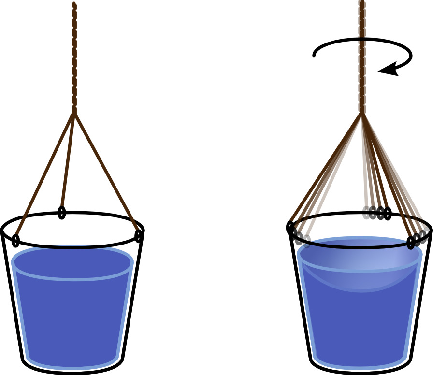
\includegraphics[width=.5\linewidth]{Figures/NewtonsBucket.png}
$$


\textcolor{vert}{\sl (Exercice classique)}  

Les surfaces de même pression (surfaces isobares) sont des paraboles 

\color{gris}{(y compris la surface libre en négligeant la tension superficielle). }



%\textbf{Théorème et poussée d'Archimède} \medskip

%On montre \textcolor{vert}{\sl (exercice)} que la résultante des efforts de pression sur la surface
%d'un corps immergé dans le champ de pesanteur est une force qui est l'opposé du poids du volume de fluide occupé par le corps, et qui s'applique au centre de gravité de ce volume de fluide, appelé centre de poussée.

%\vspace{20mm}

\end{frame}

\subsubsection{Efforts de pression sur une surface}

\begin{frame}{Efforts de pression sur une surface}

\small

Soit une surface ${\cal S}$ (matérielle ou non) délimitant 
(partiellement ou totalement) un fluide $F$ à l'équilibre.
Soit $M$  un point courant de ${\cal S}$  et 
$\vec n_{{\cal F}\rightarrow {\cal S}}$  un vecteur 
normal orienté du fluide vers la surface ("entrant").
Les efforts  exercés par $F$ sur ${\cal S}$ 
(efforts hydrostatiques) sont données par le torseur suivant :

\medskip

$$ 
\left\{ {\cal F} \rightarrow {\cal S} \right\} =  \torseur{A}{\vec R}{\vec M_{A}} =
= \torseur{A}
{\displaystyle \iint_{\cal S} p(M) \vec n_{{\cal F}\rightarrow {\cal S}} d S}
{ \displaystyle \iint_{\cal S}  \overrightarrow{ AM }\times p(M) \vec n_{{\cal F}\rightarrow {\cal S}} d S}
$$

\medskip

{\bf Remarques : }
\pause

- Dans le cas d'une surface fermée délimitant un objet $\Omega$ plongé dans le fluide, la convention habituelle est de noter 
$\vec n$ la normale sortante (par rapport à l'objet). Dans ce cas on peut utiliser les formules 
précédentes en écrivant $\vec n_{{\cal F}\rightarrow \Omega} = -\vec n$.

\pause 
- On appelle  {\em point d'application} "le" point $C$ tel que $\vec M_{C}=0$ 

(définition non rigoureuse car ce point n'est pas unique ; on peut choisir n"importe quel point situé sur la "droite d'action" du torseur).


\medskip

\textcolor{vert}{\sl Exercices classiques :} 

- Calculez la résultante des forces de pression sur un barrage rectangulaire vertical de hauteur $H$. 
Montrez que le point d'application est situé à une altitude $H/3$ par rapport au fond.

- Barrage triangulaire (exercice a préparer avant le TD, corrigé sur moodle).

\end{frame}


\subsubsection{Poussée d'Archimède}

%%%%%%%%%%%%%%%%%%%%%
\begin{frame}{Théorème d'Archimède}
\small

\pause

{\em 
"Tout corps plongé entièrement dans un ou plusieurs fluides au repos,
subit de la part du (des) fluide(s) une force verticale, dirigée 
vers le haut, égale en intensité au poids du volume de fluide 
déplacé, et qui s'applique au centre de gravité $G_f$ 
du(des) fluide(s) déplacé(s)."
}

\pause
\medskip

En termes plus précis, la poussée d'Archimède correspond au torseur suivant :

$$
\left\{ {\cal A} \right\} = \torseur{G_f}{ \vec{\cal P}_{\cal A} = -M_f \vec{g}}{ \vec{\cal M}_{{\cal A},G_f} =   \vec 0}.
$$

Démonstrations : $(i)$ physique ; $(ii)$ mathématique.

\pause
\medskip

\paragraph{\bf Remarques :}

\begin{itemize}

\item en général $G_f \neq G$ ($G$ est le centre de gravité du corps 
considéré, et dépend de la répartition de masse à l'intérieur de celui-ci). 

\item Si le fluide déplacé a une masse volumique constante $\rho_f$, alors
$M_f = \rho_f V$, et le point $G_f$ correspond au centre géométrique
$C$ de l'objet.

\item La somme de la force de gravité $M\vec g$ et de la poussée d'Archimède 
est parfois appelée "poids relatif" ou "force de flottabilité" (buoyancy) :
$\vec F = ( M - M_f ) \vec g$. 

\end{itemize}

\end{frame}



\subsubsection{Equilibre des corps flottants}


%%%%%%%%%%%%%%%%%%%%%
\begin{frame}{Equilibre des corps flottants (1)}

\small
\paragraph{\bf Cas d'un corps de masse $m$ et volume $V$ entièrement immergé dans un fluide homogène de masse volumique 
$\rho_f$ (sous-marin ou montgolfière) } 

\medskip

Recherchons les conditions d'équilibre sous l'effet de son poids $\left\{ {\cal G} \right\}$ et de la poussée d'Archimède $\left\{ {\cal A} \right\} $.

\medskip \pause 

{\bf Equilibre des résultantes :} $ m = \rho_f V$.

$ \qquad \rightarrow$ Conséquence : le véhicule doit pouvoir contrôler sa masse en fonction du milieu environnant !

\smallskip \pause

{\bf Equilibre des moments :} $ \overrightarrow{CG} \wedge m \vec g = \vec{0}$.

$ \qquad \rightarrow$ Conséquence : $C$ et $G$ doivent être alignés verticalement 

$\qquad \quad$ (position stable si $G$ est en dessous de $C$).



\end{frame}



%%%%%%%%%%%%%%%%%%%%%
\begin{frame}{Equilibre des corps flottants (2)}

\small

\paragraph{\bf Cas d'un corps de masse $m$ partiellement immergé dans un liquide homogène de masse volumique 
$\rho_f$ (bateau) } 


%Recherchons les conditions d'équilibre sous l'effet de son poids $\left\{ {\cal G} \right\}$ et de la poussée d'Archimède $\left\{ {\cal A} \right\} $.

\bigskip \pause 

{\bf Equilibre des résultantes :} $ m = \rho_f V_0$ où $V_0$ est le "volume de carène" (volume de la partie immergée)

$ \qquad \rightarrow$ Conséquence : l'équilibre reste possible si $m$ varie. 

\bigskip \pause

{\bf Equilibre des moments :} 

$$
\sum \vec{M} =  \overrightarrow{OG} \wedge m \vec{g} + \overrightarrow{OC_\phi} \wedge \vec{\cal P}_{\vec A} =  \ \overrightarrow{C_\phi G} \wedge m \vec{g} 
$$

\smallskip 
\pause

Subtilité : lorsque l'inclinaison (gîte) $\phi$ varie, le centre de carène $C_\phi$ se déplace ! 

\smallskip 
\pause

On peut montrer qu'il existe un point {\em fixe} $M$ appelé {\em Métacentre de roulis} tel que 
$\vec{\cal M}_{{\cal A},M} = \vec 0 \quad \forall  \phi$ (dans la limite $\phi \ll 1$).

\smallskip 
(cad. la droite d'action de la poussée d'Archimède passe par $M$  $\forall  \phi$) 

\smallskip
Soit :

$$\sum \vec{\cal M} =   \overrightarrow{MG} \wedge m \vec{g} \quad \forall \phi \quad \mbox{ ( dans la limite } \phi \ll 1 ) $$

\smallskip 
\pause

La position de $M$ est donné par la formule de Bouguier : 

$C_0 M = \frac{ L b^3 }{12 V_0}$ 

( pour une carène prismatique, de longueur $L$ et largeur à la flottaison $b$ ; $C_0$ étant le centre de carène de la position de référence $\phi = 0$).

\medskip \pause

$ \qquad \rightarrow$ Conséquence : la position $\phi = 0$ est stable si {\bf $G$ est en dessous de $M$.}



\end{frame}




\subsection{Tension superficielle}

%--------------------------------------------------------------------------------------------------
\begin{frame}{Tension superficielle : mise en évidence expérimentale}
%--------------------------------------------------------------------------------------------------

Expériences avec un film de savon :


%\href{https://www.math.hmc.edu/~jacobsen/demolab/soapfilm.html}{\beamergotobutton{https://www.math.hmc.edu/~jacobsen/demolab/soapfilm.html}}
%\verb|

\medskip

\href{https://www.math.hmc.edu/~jacobsen/demolab/soapfilm.html}{
 \textcolor{blue}{
https://www.math.hmc.edu/~jacobsen/demolab/soapfilm.html
}
}

\bigskip


Origami capillaire :

\medskip

%\begin{verbatim}
%\textcolor{blue}{
%https://www.youtube.com/watch?v=n51Vi3rv\_kA
%\end{verbatim}
\href{https://www.youtube.com/watch?v=n51Vi3rv_kA}{\textcolor{blue}{https://www.youtube.com/watch?v=n51Vi3rv\_kA}}
 

https://www.google.com/imgres?imgurl=http%3A%2F%2Fwww.brandeis.edu%2Fnow%2F2012%2Fjanuary%2Fimages%2Fskimmer405.jpg&imgrefurl=http%3A%2F%2Fwww.brandeis.edu%2Fnow%2F2012%2Fjanuary%2Fsurface.html&docid=rbTdmv6-P5iwCM&tbnid=m7xfpdX5vRGt8M%3A&vet=1&w=405&h=270&client=safari&bih=712&biw=1213&q=surface%20tension&ved=0ahUKEwisqaPxzrfRAhUJMhoKHRzbABo4ZBAzCAIoADAA&iact=mrc&uact=8



\end{frame}

%%%
%Quelques bons sites :

%https://fr.wikipedia.org/wiki/Tension\_superficielle
%Quelques explications fausses :

%http://www.sita-process.com/information-service/process-parameter-surface-tension/overview/


\begin{frame}{Tension superficielle : modélisation physique}

\small

\textbf{Forces linéiques : la tension de surface} \medskip

Si le volume de fluide $\Omega$ est traversé par une interface entre deux fluides non miscibles (fluide 1 et fluide 2),
le fluide contenu dans $\Omega$ est soumis à une force de tension le long de la ligne $\cal L$
intersection de la frontière de $\Omega$ avec l'interface :

\medskip

\centerline{$ \color{rouge} \displaystyle d\myvec{F}_{{\cal L} \rightarrow \Omega}  = \gamma \, dl \; \myvec{n}_{\cal L} $}
\begin{itemize}
\item[]
	o{\`u} $dl$ : longueur élémentaire le long de $\cal L$
\item[]
	et $\myvec{n}_{\cal L}$ : vecteur unitaire tangent à l'interface, $\perp$ à $\cal L$, et sortant par rapport au domaine $\Omega$
\end{itemize}

\smallskip

\pause

Le coefficient de \textcolor{rouge}{tension de surface} $\gamma$ 
correspond à une force par unité de longueur (N/m) 
\\
ou de manière équivalente à une énergie par unité de surface (J/m$^2$).



\medskip

Sa valeur est une propriété physique de l'ensemble (fluide 1/ fluide 2)
(ex. $\gamma = 0.07$ N/m pour une interface eau/air)

\pause

\medskip

{\bf  \textsl{Loi de Laplace} (rappels L2)}


\begin{itemize}
\item[]
On montre que la tension de surface conduit à un saut de pression 
de part et d'autre de l'interface :

\centerline{$ \displaystyle \color{rouge} p_1 - p_2 = \frac{2 \gamma}{\cal R} 
                                      = \gamma \, \left (\frac{1}{\cal R'}+\frac{1}{\cal R''}\right)$}
\item[]
o{\`u} $\cal R$ : rayon de courbure local de l'interface (centre de courbure dans le fluide 1)
\item[]
\myhskip{o{\`u}} $\cal R'$ et $\cal R''$ : rayons de courbure principaux en 3D (cf. cours de géométrie différentielle)
\end{itemize}


\pause

\smallskip

{\bf  \textsl{Angle de contact} (rappels L2)}

Au niveau de la ligne triple (fluide 1 / fluide 2 / paroi solide), on constate que l'angle de contact $\theta$ est fixé : $\theta = \theta_E$

$\theta_E$ est une propriété physique de l'ensemble  (fluide 1 / fluide 2 / paroi solide). 

Si $\theta_E < \pi/2$ on parle de surface hydrophile (exemple : eau/air/verre).

Si $\theta_E > \pi/2$ on parle de surface hydrophobe (exemple : eau/air/téflon).

\end{frame}

%--------------------------------------------------------------------------------------------------
\begin{frame}{Compétition entre capillarité et pesanteur}
%--------------------------------------------------------------------------------------------------

\small

\begin{overprint}

\onslide<1>   
  
\begin{center}
	\begin{picture}(60, 70)
   	\put(0, 0){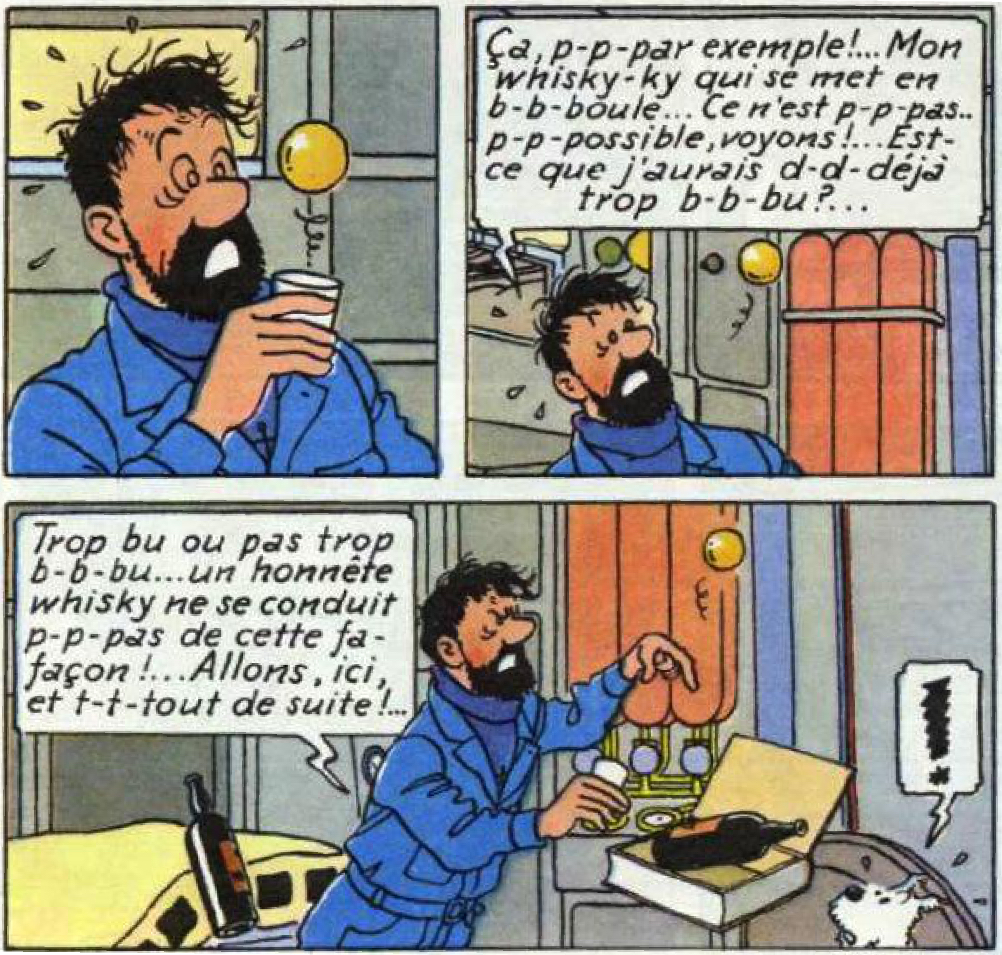
\includegraphics[height=60mm]{whisky_Haddock.jpg}}
	\end{picture}
\end{center}

\onslide<2>   

\vspace{3mm}


Le nombre sans dimension permettant de comparer gravité et capillarité est 
le nombre  de \textcolor{rouge}{\bf Bond} :

$$ \color{rouge}
\Bond = \frac{\rho g L^2}{\gamma}
$$

\medskip
o{\`u} $L$ désigne l'échelle de longueur caractéristique
du phénomène étudié 
\\
 (par ex. le diamètre du verre de whisky du Capitaine Haddock\ldots)



\bigskip

 ce nombre peut s'écrire également 
$$ \color{rouge}
\Bond = \left ( \frac{L}{\ell_c}\right )^2 
$$
où $\color{rouge} \ell_c = \sqrt{\dfrac{\gamma}{\rho g}}  $  est l'échelle de longueur capillaire.


($ \ell_c = 2.7 mm$ Pour l'interface air/eau en gravité terrestre.) 






%\pause

\begin{picture}(0, 0)
	\put(90, 15){
\includegraphics[width=20mm]{whisky_Haddock_crop.jpg}}
\end{picture}

\medskip

{\bf Interprétation :}

\medskip

\begin{itemize}
\item
	Si $\Bond \gg 1$ : pesanteur dominante (surface libre plane, horizontale).
\item
	Si $\Bond \ll 1$ : capillarité dominante (surface libre sphérique).
\item
	Si $\Bond = {\cal O}(1)$ : forces de gravité et capillarité comparables (surface libre solution d'un problème difficile...).	
	
\end{itemize}

\end{overprint}

\end{frame}

